%===============================================================================
% LaTeX sjabloon voor de bachelorproef toegepaste informatica aan HOGENT
% Meer info op https://github.com/HoGentTIN/bachproef-latex-sjabloon
%===============================================================================

\documentclass{bachproef-tin}

\usepackage{hogent-thesis-titlepage} % Titelpagina conform aan HOGENT huisstijl

%%---------- Documenteigenschappen ---------------------------------------------
% TODO: Vul dit aan met je eigen info:

% De titel van het rapport/bachelorproef
\title{Robotic Process Automation, automatisering van morgen, vandaag.}

% Je eigen naam
\author{Mout Pessemier}

% De naam van je promotor (lector van de opleiding)
\promotor{Johan Decorte}

% De naam van je co-promotor. Als je promotor ook je opdrachtgever is en je
% dus ook inhoudelijk begeleidt (en enkel dan!), mag je dit leeg laten.
\copromotor{Laurens Lavaert}

% Indien je bachelorproef in opdracht van/in samenwerking met een bedrijf of
% externe organisatie geschreven is, geef je hier de naam. Zoniet laat je dit
% zoals het is.
\instelling{Faktion}

% Academiejaar
\academiejaar{2019-2020}

% Examenperiode
%  - 1e semester = 1e examenperiode => 1
%  - 2e semester = 2e examenperiode => 2
%  - tweede zit  = 3e examenperiode => 3
\examenperiode{2}

%===============================================================================
% Inhoud document
%===============================================================================

\begin{document}

%---------- Taalselectie -------------------------------------------------------
% Als je je bachelorproef in het Engels schrijft, haal dan onderstaande regel
% uit commentaar. Let op: de tekst op de voorkaft blijft in het Nederlands, en
% dat is ook de bedoeling!

%\selectlanguage{english}

%---------- Titelblad ----------------------------------------------------------
\inserttitlepage

%---------- Samenvatting, voorwoord --------------------------------------------
\usechapterimagefalse
%%=============================================================================
%% Voorwoord
%%=============================================================================

\chapter*{\IfLanguageName{dutch}{Woord vooraf}{Preface}}
\label{ch:voorwoord}

Voor ik aan deze bachelorproef begon had ik absoluut geen idee wat \acrlong{rpa} was en wat er mee bereikt kon worden. Ik zag het dan ook al een uitdaging die ik niet links kon laten liggen om mij volledig in dit veld te gooien en de wereld van automatisatie beter te begrijpen. Wat is nu het voordeel van \acrshort{rpa} boven het schrijven van automatisatie scripts, wie bevindt zich op deze markt, hoe groot is deze markt en zit er een toekomst in.

Voordat verder gegaan wordt met deze thesis, wil ik eerst enkele mensen bedanken. Deze bachelorproef zou nooit tot stand gekomen zijn zonder de hulp van enkele mensen.\\
Eerst en vooral zou ik mijn co-promotor, Laurens Laveart, willen bedanken voor de gedetailleerde
opvolging van mijn bachelorproef. De feedback over de inhoud en de vele vragen die ik heb kunnen stellen waren cruciaal voor het succes van deze proef.\\
Verder wil ik mijn promotor, Johan Decorte, heel erg bedanken voor de uren die
gespendeerd zijn aan de opvolging van en het in goede banen sturen van deze paper.\\
Ik kan natuurlijk Jo Cijnsmans en Niels Van Weereld, het sales en marketing team van Faktion niet vergeten. Zij hebben mij ondersteund in het opstellen van het marktonderzoek dat terug te vinden is als bijlage.\\
Ik zou graag ook enkele mensen bedanken die mijn bachelorproef nog eens nagelezen hebben zoals [...] en mijn ouders.\\
Daarnaast zou ik Joeri Van Steen en Filip Martens van Faktion willen bedanken voor de mogelijkheid om op hun platform en van hun resources gebruik te mogen maken om mijn thesis tot een goed eind te brengen. \\
Bovendien wil ik nog iedereen bedanken die op de één of andere manier geholpen heeft met mijn bachelorproef.

Als laatste wens ik u nog een boeiende lectuur.


%%=============================================================================
%% Samenvatting
%%=============================================================================
\chapter*{\IfLanguageName{dutch}{Samenvatting}{Abstract}}
Als gezocht wordt naar \acrshort{rpa} aanbieders op het internet, dan wordt een lijst van providers voorzien. Hierbij heeft iedere provider wel voor- en nadelen. Om hier dan het juiste platform uit te kiezen dat past bij de bedrijfscultuur en mentaliteit is geen gemakkelijke taak. Er zijn vele aspecten die overwogen moeten worden om zo een keuze succesvol te maken. Daarom is in deze thesis onderzoek uitgevoerd geweest naar enkele van deze providers met hun sterke en zwakke punten in de hoop deze keuze makkelijker te maken of in de juiste richting te sturen.\\
Het onderzoek gaat na bij 5 providers (UiPath, Automation Anywhere, WorkFusion, IntelliBot en Microsoft Flow) waar ergens ze zich situeren in de markt, waarin ze uitblinken als platform en waaraan nog verbeteringen nodig zijn. Bij de selectie van de 5 aanbieders is rekening gehouden met grootte en soort \acrshort{rpa}. Dit is gerealiseerd geweest door met de verschillende platformen te werken om een demo proces te automatiseren en door contact te leggen met het bedrijf en de community achter de provider.\\
De hele uitwerking van elke aanbieder staat in detail beschreven in hoofdstuk drie: Methodologie. Kort samengevat, eerst is door de lessen gegaan die aangeboden worden op het platform zelf. Nadien is het proces geautomatiseerd geweest behalve de zelf geschreven activiteit. Nadien is deze activiteit geïmplementeerd en geïntegreerd geweest in de workflow. Dit is nadien extensief getest geweest op fouten.\\
Na met elk platform gewerkt te hebben, zijn aan verschillende vooropgestelde criteria punten toe gewezen. Deze criteria zijn onderverdeeld in 3 categorieën: technische-, bedrijfs- en financiële aspecten. Hoe hoger de score van de aanbieder, hoe beter.\\
De belangrijkste conclusies die uit dit onderzoek kunnen getrokken worden zijn dat UiPath ver boven de rest staat en dat de kleine providers in de toekomst waarschijnlijk uit de markt zullen verdwijnen aangezien het een race zal worden tussen de drie grote providers (UiPath, Automation Anywhere en Blue Prism) over wie de markt uiteindelijk zal beheersen. Op dit moment ziet het er naar uit dat UiPath zal winnen.\\
Mogelijke uitbreidingen op dit onderzoek zijn natuurlijk de andere providers die niet onderzocht geweest zijn. Zoals eerder vermeld is er een hele hoop aan providers waar er slechts 5 uit gekozen zijn. Een mogelijks tweede uitbreiding is dat andere criteria ook nog onderzocht kunnen worden.

%---------- Inhoudstafel -------------------------------------------------------
\pagestyle{empty} % Geen hoofding
\tableofcontents  % Voeg de inhoudstafel toe
\cleardoublepage  % Zorg dat volgende hoofstuk op een oneven pagina begint
\pagestyle{fancy} % Zet hoofding opnieuw aan

%---------- Lijst figuren, afkortingen, ... ------------------------------------

% Indien gewenst kan je hier een lijst van figuren/tabellen opgeven. Geef in
% dat geval je figuren/tabellen altijd een korte beschrijving:
%
%  \caption[korte beschrijving]{uitgebreide beschrijving}
%
% De korte beschrijving wordt gebruikt voor deze lijst, de uitgebreide staat bij
% de figuur of tabel zelf.

\listoffigures
\listoftables

% Als je een lijst van afkortingen of termen wil toevoegen, dan hoort die
% hier thuis. Gebruik bijvoorbeeld de ``glossaries'' package.
% https://www.overleaf.com/learn/latex/Glossaries

%---------- Kern ---------------------------------------------------------------

% De eerste hoofdstukken van een bachelorproef zijn meestal een inleiding op
% het onderwerp, literatuurstudie en verantwoording methodologie.
% Aarzel niet om een meer beschrijvende titel aan deze hoofstukken te geven of
% om bijvoorbeeld de inleiding en/of stand van zaken over meerdere hoofdstukken
% te verspreiden!

%%=============================================================================
%% Inleiding
%%=============================================================================

\chapter{\IfLanguageName{dutch}{Inleiding}{Introduction}}
\label{ch:inleiding}
Sinds de eerste industriële revolutie van 1750 zijn mensen op zoek naar hoe we het best verschillende processen kunnen optimaliseren en automatiseren. Er zijn al een aantal oplossingen geweest, zoals de stoommachine in de eerste industriële revolutie, elektronische apparaten tijdens de tweede industriële revolutie en natuurlijk een inleiding tot computers door Alan Turing's machine bij de derde industriële revolutie. De volgende stap in deze (r)evolutie, de vierde en huidige industriële revolutie, is dan ook \acrlong{rpa}, ook wel \acrshort{rpa} genoemd. \autocite{indusRev}

\acrshort{rpa} is waarschijnlijk het snelst en meest efficiënte pad naar de digitale transformatie. Om beter te begrijpen waarom \acrshort{rpa} hier juist zo goed in is, zal eerst besproken worden wat het is en kan doen. \acrshort{rpa} is een technologie die computer software toestaat acties die normaal gezien uitgevoerd worden door mensen te gaan simuleren of nabootsen en deze acties te integreren met digitale systemen.

\acrshort{rpa} robots, de software agenten die deze acties op zich nemen, kunnen onder andere data vastleggen, applicaties uitvoeren, antwoorden versturen, beslissingen maken gebaseerd op voorgedefinieerde regels en communiceren met andere systemen. \acrshort{rpa} is bedoeld voor processen die zeer sterk gereguleerd, repetitief en weinig uitzonderingen hebben.

\section{\IfLanguageName{dutch}{Probleemstelling}{Problem Statement}}
\label{sec:probleemstelling}
Als werknemer heel de tijd dezelfde, repetitieve taak uitvoeren is saai en vervelend werk. Als men daarbij de focus dan nog eens verliest is het ook zeer makkelijk om fouten te maken tijdens het uitvoeren van dit proces. Door het gebrek aan verantwoordelijkheid in de werknemer in combinatie met het herhaaldelijk uitvoeren van dit ene proces, verhoogt de kans op burn-outs. Om dit alles tegen te gaan kan beroep gedaan worden op \acrlong{rpa}. Hierbij zal \acrshort{rpa} voorgedefinieerde taken volledig en foutloos gaan automatiseren wat er voor zorgt dat werknemers hun tijd niet meer moeten opofferen om deze lastige taken uit te voeren maar in plaats daarvan aan nuttige en belangrijke taken kunnen werken. Dit heeft niet alleen inpakt op het mentaal welzijn van de werknemer maar ook op de kost die verminderd wordt door zo'n processen te automatiseren. Dit kan voor een bedrijf met zo een soort processen zeer voordelig uitkomen. Maar in de zee van providers kan het moeilijk worden om te weten welke nu de geschikte \acrshort{rpa} provider is.

\section{\IfLanguageName{dutch}{Onderzoeksvraag}{Research question}}
\label{sec:onderzoeksvraag}
Hoe makkelijk of juist hoe moeilijk is het om een \acrshort{rpa} workflow te integreren met een eigen webapplicatie? Welke \acrshort{rpa} provider maakt deze taak het makkelijkst en hoe zit het dan met de tijd en kost nodig voor zo een workflow uit te werken?


\section{\IfLanguageName{dutch}{Onderzoeksdoelstelling}{Research objective}}
\label{sec:onderzoeksdoelstelling}
Uit het onderzoek zal een duidelijk beeld naar boven komen wat de voor en nadelen zijn van enkele gekozen \acrshort{rpa} providers om een integratie met een webapplicatie te voorzien. Hierbij zal rekening gehouden worden met kost van de service, implementatie tijd en gemak van integreren.

\section{\IfLanguageName{dutch}{Opzet van deze bachelorproef}{Structure of this bachelor thesis}}
\label{sec:opzet-bachelorproef}
De rest van deze bachelorproef is als volgt opgebouwd:

In Hoofdstuk~\ref{ch:stand-van-zaken} wordt een overzicht gegeven van de stand van zaken binnen het onderzoeksdomein, op basis van een literatuurstudie.

In Hoofdstuk~\ref{ch:methodologie} wordt de methodologie toegelicht en worden de gebruikte onderzoekstechnieken besproken om een antwoord te kunnen formuleren op de onderzoeksvragen.

In Hoofdstuk~\ref{ch:conclusie}, tenslotte, wordt de conclusie gegeven en een antwoord geformuleerd op de onderzoeksvragen. Daarbij wordt ook een aanzet gegeven voor toekomstig onderzoek binnen dit domein.
\chapter{\IfLanguageName{dutch}{Stand van zaken}{State of the art}}
\label{ch:stand-van-zaken}

% Tip: Begin elk hoofdstuk met een paragraaf inleiding die beschrijft hoe
% dit hoofdstuk past binnen het geheel van de bachelorproef. Geef in het
% bijzonder aan wat de link is met het vorige en volgende hoofdstuk.

% Pas na deze inleidende paragraaf komt de eerste sectiehoofding.

%Dit hoofdstuk bevat je literatuurstudie. De inhoud gaat verder op de inleiding, maar zal het onderwerp van de bachelorproef *diepgaand* uitspitten. De bedoeling is dat de lezer na lezing van dit hoofdstuk helemaal op de hoogte is van de huidige stand van zaken (state-of-the-art) in het onderzoeksdomein. Iemand die niet vertrouwd is met het onderwerp, weet nu voldoende om de rest van het verhaal te kunnen volgen, zonder dat die er nog andere informatie moet over opzoeken \autocite{Pollefliet2011}.

%Je verwijst bij elke bewering die je doet, vakterm die je introduceert, enz. naar je bronnen. In \LaTeX{} kan dat met het commando \texttt{$\backslash${textcite\{\}}} of \texttt{$\backslash${autocite\{\}}}. Als argument van het commando geef je de ``sleutel'' van een ``record'' in een bibliografische databank in het Bib\LaTeX{}-formaat (een tekstbestand). Als je expliciet naar de auteur verwijst in de zin, gebruik je \texttt{$\backslash${}textcite\{\}}.
%Soms wil je de auteur niet expliciet vernoemen, dan gebruik je \texttt{$\backslash${}autocite\{\}}. In de volgende paragraaf een voorbeeld van elk.

%\lipsum[7-20]

\acrshort{rpa} is een onderdeel van business process automation (BPA), een overkoepelende term gebruikt voor het beschrijven van technologieën die activiteiten en workflows waaruit business taken bestaan uitvoeren met zo min mogelijk menselijke tussenkomst. \autocite{everythingRPA}

RPA kan gecombineerd worden samen met artificiële intelligentie om zo langere en moeilijkere taken op zich te nemen. Hierdoor worden ze door sommigen beschreven als zelf-verbeterende digitale werkkrachten. Enkele velden waarbinnen RPA kan gecombineerd worden met AI zijn optical character recognition en natural language generation (NLG). \autocite{everythingRPA}

\section{Algemene informatie}

\subsection{Waarvoor kan RPA gebruikt worden}
Enkele taken waarvoor RPA kan worden gebruikt:
\begin{itemize}
	\item data overzetten van de ene applicatie naar de andere
	\item processen automatiseren
	\item website scraping
	\item data verzamelen en analyseren
	\item reporting
	\item emails verzenden
	\item werken met spreadsheets, PDFs, texteditors
\end{itemize}
\autocite{everythingRPA} \autocite{idrRPA}

\subsection{In welke sectoren wordt RPA gebruikt}
Onderdelen van een onderneming waarbinnen deze taken kunnen gebruikt worden:
\begin{itemize}
	\item klantenservice: validatie van handtekeningen, uploaden van ingescande documenten, valideren van informatie voor automatische aanvaarding of afwijzing
	\item accounting: procedure to pay, accounting, belastingen
	\item human resources (HR): payroll, time management, recruitment
	\item IT management en services: source-code control management, incident management, optimaliseren van e-mail notificaties
	\item supply chain management: order processing, payment processing, monitoring van de stock
\end{itemize}
\autocite{everythingRPA}

\subsection{Welke processen kunnen geautomatiseerd worden}
RPA is kan niet gebruikt worden om zo maar eender welk business proces te gaan automatiseren. Een proces toont best een aantal karakteristieken die het geschikt maken om te automatiseren:
\begin{itemize}
	\item repetitief
	\item gebaseerd op gestructureerde, digitale data
	\item duidelijk afgebakende regels met weinig tot geen uitzonderingen
	\item error-prone als het uitgevoerd wordt door een werknemer
	\item tijdsgebonden
\end{itemize}

\subsection{Automation-First gedachtegang}
In de Automation-First gedachtegang moet je elk bedrijfsproces kritisch bekijken met de gedacht of het niet automatiseerbaar is. Deze gedachtegang overnemen en toepassen binnen het eigen bedrijf is de eerste stap op de weg naar het maken van de digitale transformatie binnen het bedrijf. Werken via deze Automation-First mindset zorgt ervoor dat bedrijven zicht sneller en efficiënter kunnen bewegen. Het neemt alledaagse lasten weg van de werknemers om zo meer tijd vrij te maken voor het oplossen van complexe en uitdagende problemen.

Het overnemen van een automation-first mindset is de eerste stap naar het inzetten van een digitale transformatie in een onderneming. Denken op die manier staat toe aan een organisatie om sneller en meer efficiënt te bewegen binnen de sector door onder andere te helpen met het verhogen van de klantenservice of beter te kunnen inspelen op marktwijzigingen en meer efficiënt te kunnen werken.

\section{Verschillen met soortgelijke technologieën}

\subsection{Gewone automatisatie}
Het grote verschil tussen RPA en gewone automatisatie is de kennis van coderen die nodig is om het doel te bereiken. Bij gewone automatisatie schrijft een programmeur code die een bepaalde taak automatiseert. Bij RPA daarentegen wordt over het algemeen weinig tot geen code gebruikt om een proces te gaan automatiseren.

\subsection{Business Process Management}
Ook is er een verschil tussen RPA en business process management (BPM). Beide willen het aantal fouten verminderen en efficiëntie verhogen maar ze doen dat op faliekant andere manieren. BPM gaat helderheid scheppen bij business processen door deze te gaan modelleren en in kaart te brengen waar RPA deze processen juist wil gaan automatiseren, daarom niet in kaart brengen.

\subsection{Intelligent Process Automation}
Als laatste is er intelligent process automation (IPA) tegenover RPA. Er is hier minder sprake van een verschil aangezien IPA RPA combineert met BPM, AI en machine learning (ML) om processen optimaal te gaan verbeteren.
\autocite{everythingRPA}

\section{De verschillende RPA Architecturen}
Er zijn verschillende soorten RPA die kunnen gebruikt worden binnen een bedrijfscontext:

\begin{itemize}
	\item Assisted (Attended) automation: RPA loopt op een gebruiker zijn desktop om hem te helpen een proces op een snellere manier kunnen af te werken. Dit leidt in het algemeen tot een vermindering van kosten en een betere klantenservice. Een groot nadeel aan deze architectuur is dat een wijziging of onregelmatigheid in de beeldscherm instellingen zoals het wijzigen van display instellingen als lettergrootte kan er voor zorgen dat RPA faalt in het uitvoeren van de vooropgestelde taak.
	\item Unassisted (Unattended) automation: heeft geen menselijke interactie nodig, RPA draait het systeem zelf en laat pas iets weten aan de werknemer wanneer iets fout gaat en hij het zelf niet kan oplossen. Dit zijn de 24/7 digitale werkkrachten die geassocieerd worden met RPA.
	\item Hybrid RPA: Een combinatie van vorige 2 architecturen waarbij de werknemer en de RPA robot als een team samen werken, onderling taken van en naar elkaar sturen. De hybride methode overkoepelt op deze manier zowel het werk dat alleen uitgevoerd kan worden door de robot als ook het werk waarvoor menselijke interactie nodig is.
\end{itemize}

Daarnaast kan RPA op verschillende manieren geïmplementeerd worden, zo kan de low-code development mentaliteit gevolgd worden waarbij amper iets van kennis nodig is. Dit is perfect voor bedrijven met een beperkte IT kennis. Aan de andere kant kan ook veel gecodeerd worden om deze robots op te zetten.
\autocite{everythingRPA}

\section{Voordelen van RPA}

\subsection{Efficiëntie}
Vanwaar komt de efficiëntie van RPA?
\begin{itemize}
	\item Robots werken 24/7: in tegenstelling tot werknemers blijven robots werken na de werkuren. Ze worden ook niet moe en moeten nooit naar de wc. Ze kunnen ook hun concentratie niet verliezen. Als al deze punten opgeteld worden, dan kan slechts 1 conclusie getrokken worden: RPA robots zijn harde werkers die nooit pauze nodig hebben.
	\item Snellere uitvoertijd: het aantal transacties die een robot kan afwerken per uur is veel meer dan het aantal dat een werknemer ooit zou kunnen afwerken binnen hetzelfde tijdskader.
	\item Het vinden van fouten in het systeem: RPA verzamelt informatie over het systeem waar het op werkt en giet dit in een analytisch overzicht. Hier kan nadien informatie uit gehaald worden waar een vertraging of opstopping in het proces zich voordoet.
	\item Meer gemotiveerde werknemers: waar RPA het proces zal verbeteren, zal ook de werknemer die verlost is van deze lastige taak meer motivatie tonen naar de leuke processen waaraan deze nu kan werken.
	\item Doe meer met minder: Waar RPA kan gezien worden als een manier om even veel werk te verrichten met minder werknemers is het beter om te kijken naar de mogelijkheden die RPA biedt om meer werk te verrichten met hetzelfde aantal werknemers wat tot een groei van de onderneming kan leiden.
\end{itemize}

\autocite{efficiencyRPA}
\subsection{Nauwkeurigheid}
Als een proces juist opgezet is, dan kunnen RPA robots dit proces blijven juist uitvoeren zonder vermoeid te raken, hierdoor daalt het foutpercentage drastisch tot dicht bij 0\%. \autocite{efficiencyRPA}

\subsection{Kostvermindering}
RPA zorgt ervoor dat de hoeveelheid werk die afgewerkt geraakt zal stijgen met eenzelfde aantal werknemers of staat toe aan een bedrijf om met minder werknemers even veel werk klaar te krijgen. \autocite{efficiencyRPA}

\subsection{Werknemer productiviteit en moraal}
Door werknemers van de saaie en repetitieve taken weg te nemen en ze te laten werken aan taken die wel degelijk belang hebben binnen een bedrijf stijgt de inzet, moraal en productiviteit die van een werknemer kan verwacht worden. \autocite{efficiencyRPA}

\subsection{Digitale transformatie}
Door het gebruik van RPA kan een bedrijf delen of hele processen gaan automatiseren zonder wijzigingen aan te brengen aan legacy-code of te investeren in integratie van back-end systemen met reeds bestaande systemen. Hierdoor kunnen ze verder door gaan in deze digitale transformatie. \autocite{efficiencyRPA}

\section{Nadelen van RPA}
Gemiddeld falen 30 tot 50\% de eerst RPA projecten. \autocite{everythingRPA} Een van de grootste redenen waarom zo veel projecten falen is het feit dat men denkt dat een RPA project een puur IT project is. Dit is niet correct, het RPA proces moet opgezet worden door werknemers die kennis hebben van RPA maar ook de werknemers die het proces snappen en de 'as-is' kunnen interpreteren om zo deze werknemers te sturen in de juiste richting.

Enkele andere veelvoorkomende risico's zijn:

\subsection{Onderschatten van human capital}
Ondanks net gezegd dat RPA niet alleen IT is, is de aanwezigheid van IT van vitaal belang om een RPA project te kunnen blijven ondersteunen/onderhouden. Iedereen kan een proces automeren maar het draaiende houden en onderhouden is al een pak technischer en dus niet voor iedereen weggelegd. \autocite{everythingRPA}

\subsection{Security risico's}
RPA brengt een aantal security risico's met zich mee. Zo kan een robot die niet goed geïmplementeerd is bijvoorbeeld frauduleuze zaken uitvoeren of toegang krijgen tot en werken met sensitieve data en beheerders privileges gaan misbruiken. Het is dus belangrijk om de processen zorgvuldig en aandachtig te gaan opstellen en zeker te controleren dat deze risico's vermeden kunnen worden. \autocite{everythingRPA} \autocite{predictionRPA}

\section{Moeilijkheden van RPA}
RPA moet gebruikt worden om de juiste processen te gaan automatiseren, maar wat zijn nu de juiste processen? Bedrijven lijken het zeer moeilijk te vinden om die processen aan te duiden die werkelijk baat hebben moesten ze geautomatiseerd worden. Hierbij komt meestal nog eens kijken dat business de bots implementeren zonder echt te snappen wat ze doen of dat IT de processen automatiseert zonder deze echt te snappen. Dit leidt tot het repliceren van inefficiëntie maar dan op snelheid.  \autocite{cFutRPA}

Een manier om dit op te lossen is door gebruik te maken van process mining. Deze technologie maakt gebruik van business data en gebruiker interactie data om een duidelijk beeld te geven wat en hoe processen nu werkelijk in elkaar zitten en gebruikt worden. Elke stap die genomen wordt tijdens het proces wordt vastgelegd en gebruikt om dit beeld verder op te bouwen. Dit zorgt voor een grotere verstandhouding rond het proces en zorgt ervoor dat bedrijven de wrijving binnen de loop van een proces kunnen identificeren en verbeteren. \autocite{cFutRPA}

\subsection{Meest gemaakte fouten}
Naast het succes blijkt het implementeren van RPA toch niet zo eenvoudig. Zo faalde meer dan 40\% van de projecten op een van volgende 4 punten:
\begin{itemize}
	\item implementatie tijd
	\item implementatie kost
	\item het verminderen van kosten door RPA
	\item voordeel bij het uitvoeren van analyses
\end{itemize}

Er zijn heel wat verschillende zaken die aan de oorzaak van het falen van een RPA project kunnen liggen. \autocite{pitfallsRPA}

\subsubsection{Fouten op organisatie niveau}
Op eenzelfde lijn zitten, eenzelfde gedachte gang binnen een organisatie is een sleutel aspect tot succes. Als dit niet het geval is, treden enkele veelvoorkomende fouten op. Zo zijn de grootse fouten op organisatie niveau het niet genoeg ondersteunen van het RPA project. Hierdoor is er te weinig IT ondersteuning om het proces te implementeren of het leiderschap dat niet achter het project staat. Ook is er kans dat het team te weinig tijd in het project steekt. Het is van uitermate belang dat iedereen eenzelfde visie deelt over het project en dat iedereen binnen de organisatie er achter staat. \autocite{pitfallsRPA}

\subsubsection{Fouten op proces niveau}
De meest belangrijke beslissing is welk proces nu zal geautomatiseerd worden. Hier zitten dan ook de grootste fouten op proces niveau. Zo wordt er vaak gekozen om processen te automatiseren die zeer frequent wijzigen of weinig tot geen business waarde opleveren. Ook wordt geregeld een proces gekozen dat cognitieve beslissingen nodig heeft om te werken of te complexe processen bevat. RPA biedt geen oplossing voor dit soort problemen. Hiervoor moet al gekeken worden naar RPA 2.0 of IPA. \autocite{pitfallsRPA}

\subsubsection{Fouten op implementatie niveau}
Op implementatie niveau zit de grootste fout dat men alles intern wil houden. Een eigen team die een eigen oplossing zoekt voor een (veelvoorkomend) proces. Het is niet verkeerd om beroep te doen op RPA experts die kunnen helpen met het opzetten van agenten. \autocite{pitfallsRPA}

Daarnaast wordt geprobeerd om elk proces voor 100\% te automatiseren. Dit kan nadelig uitvallen aangezien 80\% makkelijk te automatiseren is maar die laatste 20\% juist zeer moeilijk en duur. In deze gevallen is het beter om die laatste 20\% toch te laten uitvoeren door een werknemer. \autocite{pitfallsRPA}

\subsubsection{Fouten op technisch niveau}
De meest voorkomende fouten op technisch niveau gaan over het kiezen van te programmeer intensieve oplossingen die niet schaalbaar zijn. In plaats hiervan kan gekeken worden naar RPA marketplaces. \autocite{pitfallsRPA}

RPA is een evoluerende sector. Het is belangrijk dat de laatste trends gevolgd worden en processen geoptimaliseerd blijven door nieuwe technieken. Hier schuilt het gevaar dat oplossingen gekocht worden op RPA marktplaatsen om tijd uit te sparen. Nadien blijkt dan dat de gekochte oplossing outdated is en helemaal niet meer zo efficiënt. Hierdoor is de onderneming zowel tijd als geld kwijt aan een suboptimale oplossing. \autocite{pitfallsRPA}

\subsubsection{Fouten na het implementeren}
Het verhaal van RPA stopt niet eens de agent online is en het werk uitvoert. Ook onderhoud en schaalbaarheid zijn van belang. Men ziet dan ook dat er velen de RPA service links laten liggen eens deze werkt wat resulteert in extra kosten maar ook een vertraging van de digitale transformatie van een organisatie. \autocite{pitfallsRPA}

\section{De toekomst van RPA}
We hebben natuurlijk geen glazen bol en kunnen dus niets met zekerheid zeggen over de toekomst van RPA. Wel kan gespeculeerd worden hoe deze technologie zal evolueren in de komende jaren. Experten zijn het er over het algemeen mee eens dat RPA de toekomst is van automatisering binnen IT. \autocite{futRPA}

\subsection{Enkele nummers}
RPA is ver gekomen sinds 2016. Toen lag het bedrag van gekochte RPA software rond \$73 miljoen. Dit is gestegen tot \$113 miljoen in 2017, \$153 miljoen in 2018 en \$192 miljoen in 2019. Er wordt geschat dat dit bedrag zal stijgen tot \$232 miljoen in 2020 en tegen 2021 zou dit bedrag liggen rond de \$272 miljoen. Hieruit valt duidelijk af te leiden dat er een sterke stijging in het gebruik van RPA voorlopig aan de gang is en dat dit niet direct blijkt te stoppen. Meer en meer ziet men dat RPA in de globale markt opgenomen wordt. \autocite{futRPA} Ondanks dat de enorme groei in RPA uitgaven blijft stijgen, zijn er toch enkele vragen die op komen rond de levensduur van RPA-markten. \autocite{everythingRPA}

Enkele verwachtingen:
\begin{itemize}
	\item Meer gebruik in de komende jaren door het leggen van de focus op de no-code/low-code oplossingen 
	\item combinatie met AI, cloud services en ML om RPA te verheven tot IPA
	\item combinatie met andere tools
	\item RPA marktplaatsen: geen enkele RPA software aanbieder kan alle in gebruikte processen ondersteunen. Door het oprichten van RPA marktplaatsen kunnen software bedrijven zelf extensies en plugins schrijven en deze verkopen
\end{itemize} \autocite{futureRPA}\autocite{everythingRPA}

\subsection{RPA 2.0}
RPA 2.0, ook wel intelligent digital robots (IDR) genoemd, gaat de huidige RPA gaan verbeteren door gebruik te maken van AI en ML om de robots slim te maken. Hierdoor moeten ze niet blindelings de regeltjes volgen maar kunnen ze, gebaseerd op de algoritmen en de interpretatie van de data, eigen beslissingen maken. Dit is een duidelijke stap naar het befaamde IPA. \autocite{idrRPA}

Vooral deep-learning en reinforcement learning technieken worden gebruikt om RPA 2.0 te verwezenlijken. \autocite{idrRPA}

\subsection{Hyperautomation}
Hyperautomation gaat RPA combineren met ML, AI en andere disruptieve technologieën om een end-to-end automatisatie oplossing te vinden die meer impactvol is dan traditionele RPA of automatisatie. Deze verzameling van technologieën speelt dan ook perfect in op de automation-first mindset die een goedde RPA ontwikkelaar nodig heeft om de juiste processen te kunnen automatiseren met succes. \autocite{hyperautomation}

\subsection{IPA}
Intelligent Process Automation gaat RPA gaan combineren met onder andere AI en ML technieken om aan de software agent toe te staan dat hij complexere processen kan gaan automatiseren waarbij enige vorm van beslissingen maken nodig is.

IPA omvat 5 technologieën:
\begin{itemize}
	\item RPA: een software automatisatie tool die routinematige taken zoals data extractie en opschoning automatiseren door een grafische gebruikers interface.
	\item Smart workflow: een process-management software tool die taken uitgevoerd door zowel man als machine integreert.
	\item ML: algoritmen die patronen in herkennen in data zoals dagelijkse performantie data. Dit gebeurd aan de hand van gesuperviseerd of ongesuperviseerd leren. Bij gesuperviseerd leren is de data gelabeld en wordt deze data gebruikt om voorspellingen te doen over nieuwe data. Bij ongesuperviseerd leren is de data niet gelabeld. Deze algoritmen worden onder andere gebruikt bij het herkennen van clusters in de data.
	\item NLG: software engines die vlotte interacties tussen mensen en technologie maken door het volgen van regels om observaties van data te vertalen [into prose?].
	\item Cognitive agents: technologieën die ML en NLG combineren om compleet virtuele werkkrachten of agenten te maken die in staat zijn om taken uit te voeren, communiceren, leren van datasets en zelfs beslissingen maken gebaseerd op de interpretatie van emoties.
\end{itemize}

Enkele puntjes om in het achterhoofd te houden hoe het best IPA geïmplementeerd wordt:
\begin{itemize}
	\item Beslis snel welke rol het IPA model speelt in het operationele model: snap het proces en de weg die afgelegd moet worden.
	\item Ontwerp oplossingen rond het volledige IPA portfolio om zo de impact te maximaliseren: IPA is het sterkst wanneer alle technologieën gecombineerd worden, bedrijven moeten hier dan ook gebruik van maken en zicht niet bezig houden met slechts enkele van de technologieën.
	\item Bouw het minimum viable product (MVP) snel: in plaats van jaren te werken aan het product om het perfect te krijgen en zo eventueel over tijd en/of budget te gaan, kan beter de focus gelegd worden op het afwerken van een MVP die simpele taken al kan oplossen waarop IPA kan toegepast worden. Dit zal namelijk al waarde creëren terwijl de meer uitgebreide versie afgewerkt wordt.
	\item bouw momentum op en leg waarde vast: denk zowel aan de kleine overwinning op de weg als aan de  lange termijn doelstellingen.
\end{itemize} \autocite{everythingIPA}

Hieruit kan makkelijk de conclusie getrokken worden dat de groei van RPA in de komende jaren alleen maar zal toenemen. Dit is daarom niet noodzakelijk in de vorm van alleenstaande RPA oplossingen maar ook bijvoorbeeld in tussenstappen zoals RPA 2.0 of hyperautomation naar IPA.
%%=============================================================================
%% Methodologie
%%=============================================================================

\chapter{\IfLanguageName{dutch}{Methodologie}{Methodology}}
\label{ch:methodologie}

Aan de hand van verschillende \acrshort{rpa} providers zal een concreet proces geautomatiseerd worden op MetaMaze. MetaMaze is een \acrfull{adp} tool ontwikkeld door Faktion. De code voor de verschillende workflows en packages geschreven voor dit onderzoek zijn te vinden op GitHub\footnote{https://github.com/MoutPessemier/BachelorProef}. Aan de hand van de uitwerking van dit proces worden de verschillende platformen gequoteerd. Deze score is een indicator hoe professioneel en gebruiksvriendelijk elk van de onderzochte platformen zijn.

Het onderzoek werd gestart vanuit het perspectief van een beginnende \acrshort{rpa} ontwikkelaar. De ervaring rond het werken met de verschillende \acrshort{rpa} providers kan sterk verschillen met een ervaren developer.


\section{Voorbereiding}
Eerst en vooral is het MetaMaze platform grondig geëxploreerd geweest. Zo werd een nieuw project aangemaakt, werden er documenten geüpload en gelabeld om een model te kunnen trainen. Nadien werd dit model dan gebruikt om voorspellingen te doen op nieuwe, soortgelijke documenten. Hierbij werd soms doelbewust een verkeerd document geüpload om ook de manuele interventie te testen en te kijken hoe dit eventueel in een proces kan gegoten worden. Op basis hiervan werd een algemeen voorbeeld proces opgezet.

Als tweede stap is de afweging gemaakt welke providers vergeleken gingen worden. Hierbij werd rekening gehouden dat er twee grote marktspelers, twee kleine en een provider die de implementatie van \acrshort{rpa} op een totaal andere manier aanpakt, gekozen waren. De volgende providers werden uiteindelijk gekozen: UiPath, Automation Anywhere, WorkFusion, IntelliBot en Microsoft Flow. Hierbij zijn Uipath en Automation Anywhere de grote providers, WorkFusion en IntelliBot de kleine en Microsoft Flow als ander concept.

 Nadien werd de documentatie en cursussen van deze platformen grondig bekeken om uiteindelijk een demo proces te bekomen. De uitwerking hiervan is te zien in figuur ~\ref{fig:exampleProcess}.

\begin{figure}[h]
	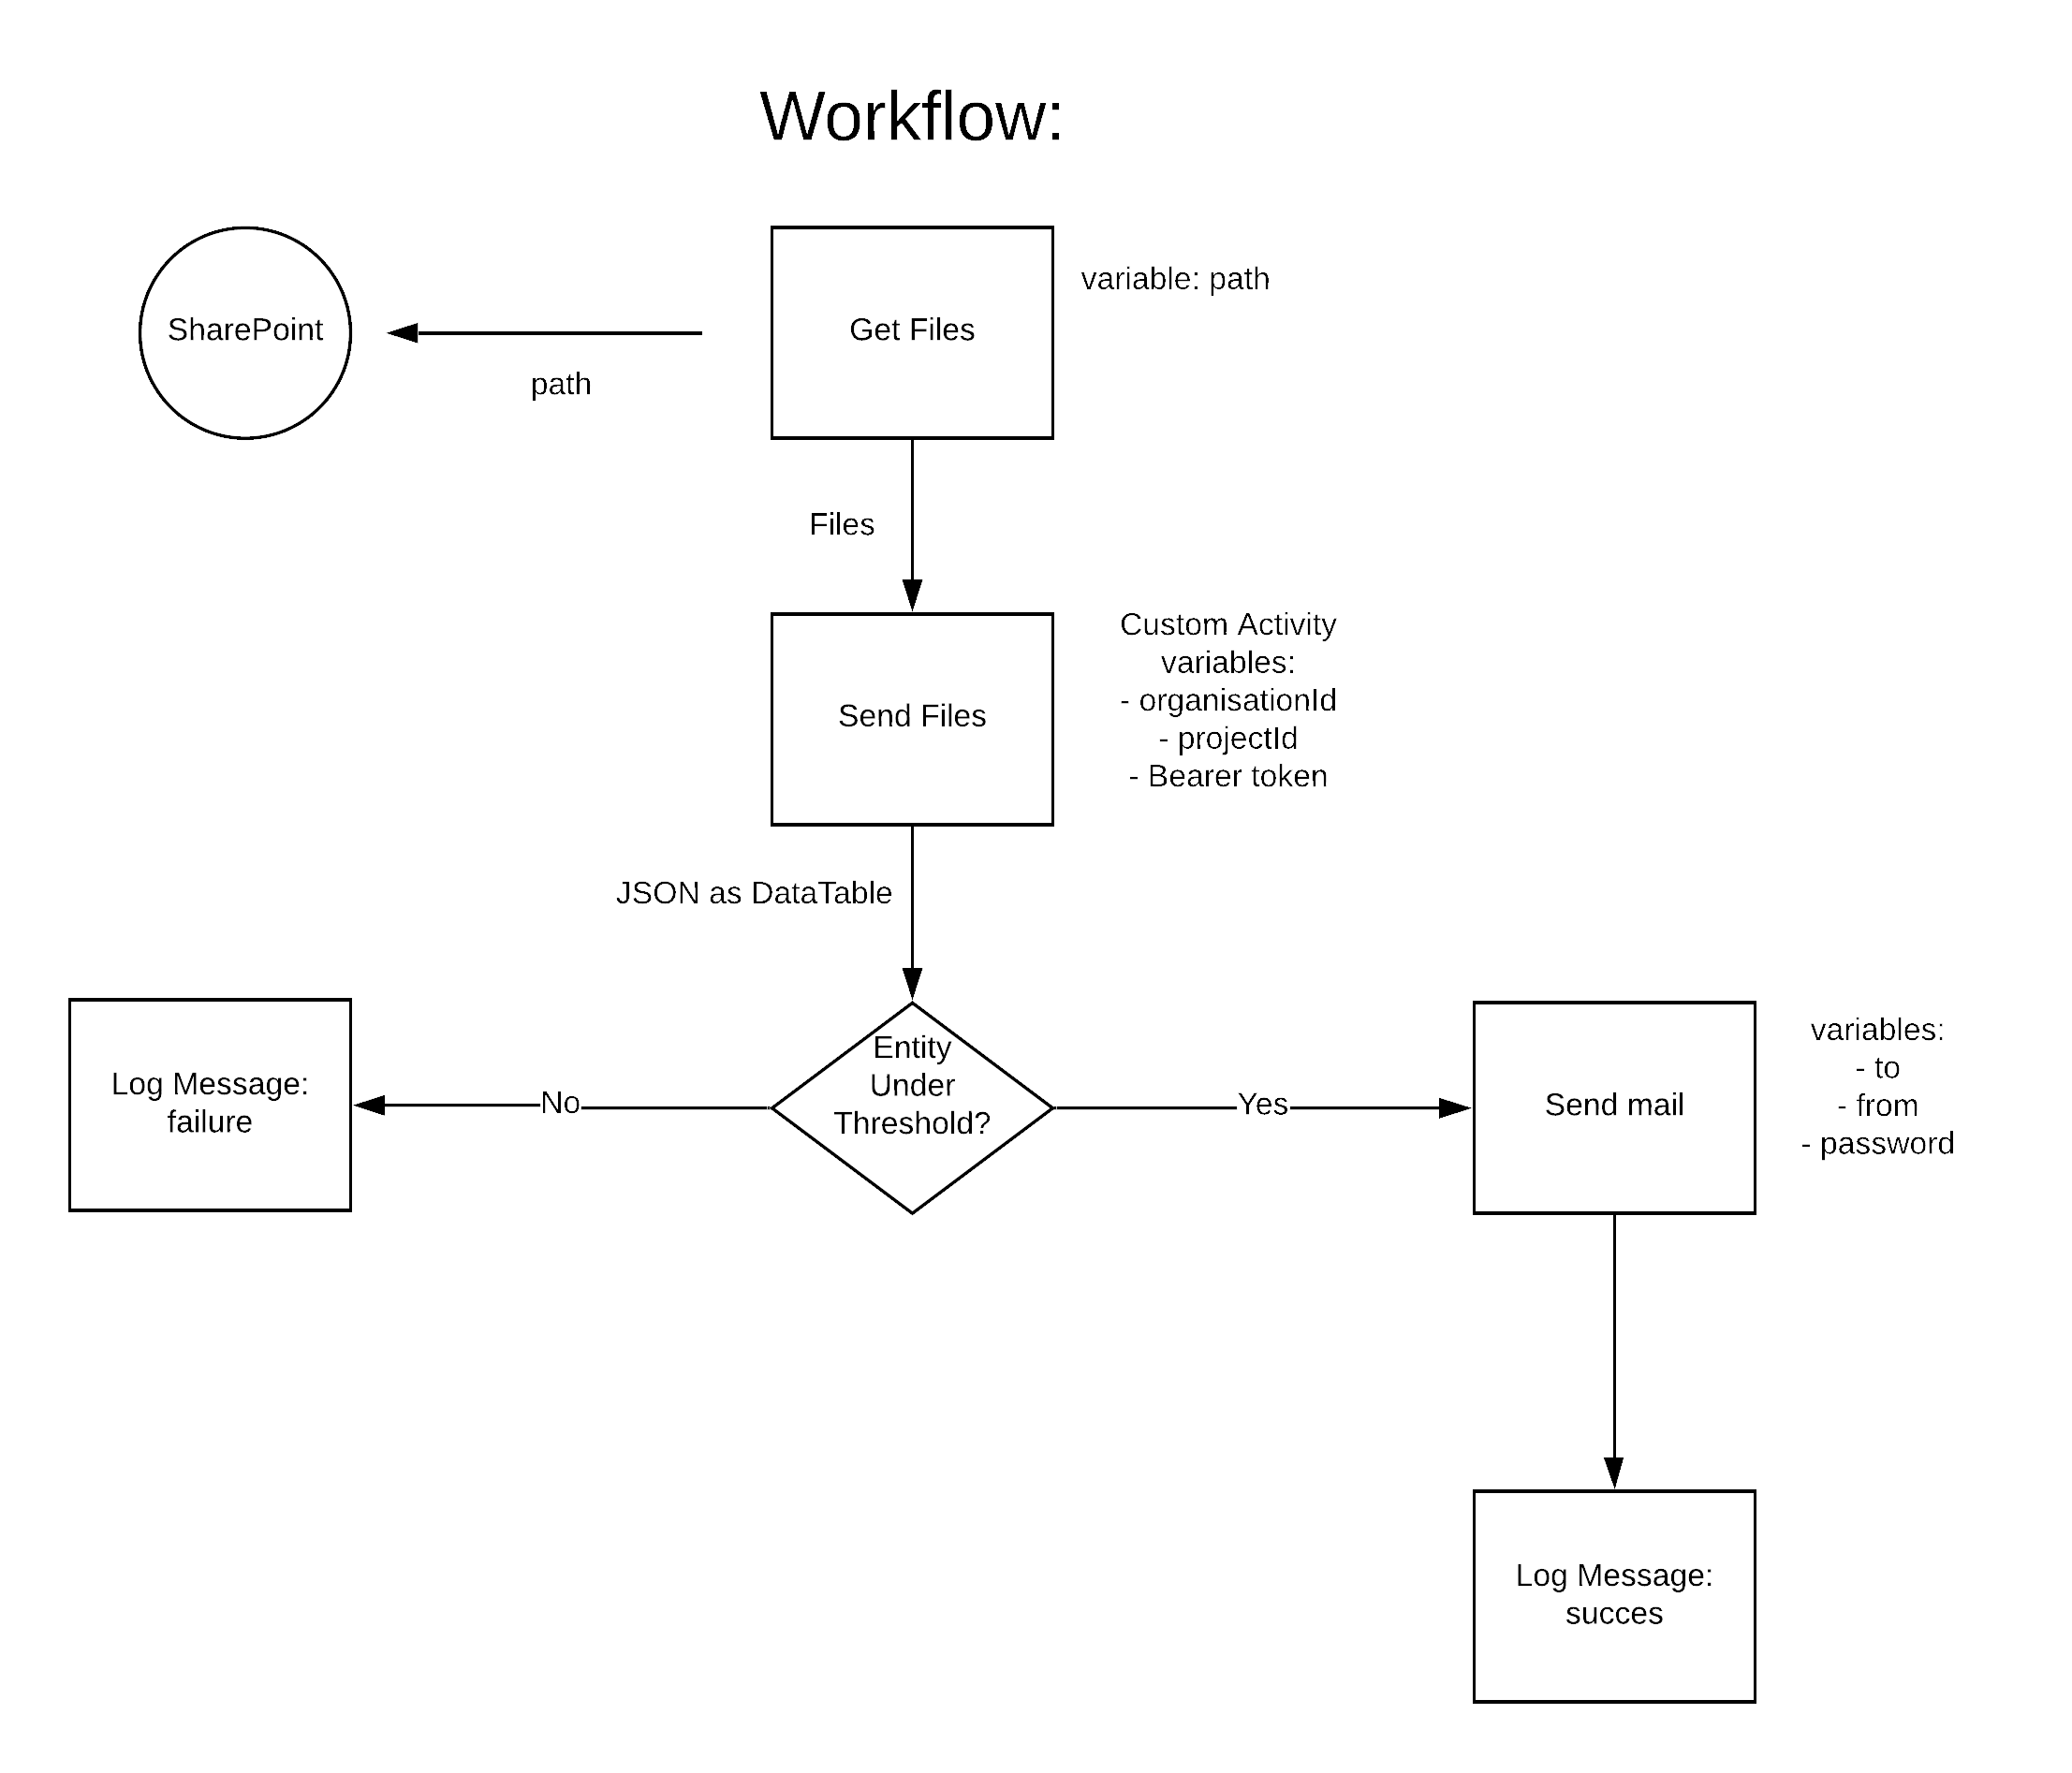
\includegraphics[width=\linewidth]{ExampleProcess.png}
	\caption[Te automatiseren demoproces]{Voorbeeldproces dat gebruik maakt van de custom Send Files \gls{activiteit}.}
	\label{fig:exampleProcess}
\end{figure}

Het algemeen proces dat zal geautomatiseerd worden op de verschillende \acrshort{rpa} solutions gaat als volgt te werk: Eerst wordt vanuit een bepaald punt (folder op de computer, OneDrive, DropBox, SharePoint) een aantal files opgehaald. Deze files worden doorgegeven aan een zelfgeschreven \gls{activiteit}. In deze \gls{activiteit} zullen deze files verstuurd worden naar de MetaMaze \acrshort{api}. De bestanden worden door de backend verwerkt. Nadien wordt er gewacht tot een antwoord terug komt van de server met de resultaten van de upload. Deze resultaten worden terug gegeven naar de volgende stap in de \gls{workflow}. Door verder te werken met de resulterende \acrshort{json} kan gekeken worden of de zekerheid waarmee een bepaalde entity dat uit een document is gehaald, onder de minimum zekerheid (threshold) zit of niet. Als er geen waarden onder de threshold zitten wordt het proces afgesloten met een gepaste melding. Als er één of meerdere confidence scores onder de threshold zitten zal eerst een mail verstuurd worden naar de klant om deze te informeren welke entities de minimum score niet gehaald hebben, voor dat het proces eindigt met een gepaste melding.

Dit is echter slechts een voorbeeldproces dat gebruikt wordt om de capaciteiten voor algemene taken zoals het versturen van een mail en werken met het bestandssysteem van de host te gaan onderzoeken.

\subsection{Criteria}
De criteria die onderzocht zijn kunnen opgedeeld worden in drie categorieën: technische criteria, bedrijfscriteria en financiële criteria.\\
Onder de technische criteria valt de mogelijkheid om zelfgeschreven \gls{activiteit}en gemakkelijk toe te voegen of te hergebruiken. Ook wordt er gekeken naar hoe het zit met de tools om de \gls{workflow}s te maken en de bots te managen. Als laatste punt wordt gekeken naar de \acrshort{ipa} capaciteiten.\\
Bij de bedrijfscriteria wordt rekening gehouden met het feit of er een grote onderneming achter het platform staat, hoe actief de community is en hoe professioneel de klantservice is.\\
Tot slot valt onder de financiële categorie de prijs van een enterprise versie maar daarnaast de mogelijkheid om een community editie te gebruiken en hoe uitgebreid deze versie is.

De nadruk wordt hier gelegd op een integratie met een eigen \acrshort{api}, op een eigen webplatform.

De verschillende criteria hebben elk een gewicht toegekend gekregen. Hierop worden ze gescoord en op het einde worden alle punten opgeteld.

\subsubsection{Puntenverdeling}
Technische Criteria
\begin{itemize}
	\item Custom activities/implementations --> is de mogelijkheid er om een eigen code toe te voegen. Als die er is, hoe uitgebreid is dit, enkel als script of ook volwaardige \gls{activiteit}en: /5
	\item Herbruikbaarheid --> kunnen bepaalde (zelfgemaakte) \gls{workflow}s/activities hergebruikt worden door jezelf en/of anderen: /3
	\item Tools --> hoe uitgebreid zijn de tools om een \gls{workflow} op te zetten: /5
	\item Bot management --> hoe en waar worden de bots gemanaged? Kan dit op een efficiënte manier: /3
	\item IPA capaciteiten --> kan \acrshort{ai} en \acrshort{ml} makkelijk geïntegreerd worden in de \gls{workflow} om IPA te bereiken. Wat wordt aangeboden door de provider zelf: /3
\end{itemize}

Bedrijfscriteria
\begin{itemize}
	\item Community --> hoe actief zijn ze op het forum, hoe groot is de community: /5
	\item Weblessen --> worden weblessen aangeboden door de provider en wat is de kwaliteit van deze lessen: /3
	\item Support --> hoe is het contact met de organisatie: /3
\end{itemize}

Financiële criteria
\begin{itemize}
	\item Prijs --> Wat is de prijs is het platform
	\item Community edition --> hoe uitgebreid en representatief is deze versie ten opzichte van de enterprise edition: /5
\end{itemize}

Dit komt uit op een totale score van 34.

\section{Implementatie}
Voor de implementatie op elk platform werd eenzelfde werkwijze gehanteerd. Eerst werd de \gls{workflow} opgebouwd rond de zelfgeschreven \gls{activiteit} om deze nadien te implementeren in de achterliggende programmeertaal van het platform. Eens deze uitgeschreven was, werd uitgezocht hoe deze \gls{activiteit}en gebruikt konden worden binnen de verschillende \gls{workflow}s.

Voor de uitwerking van de zelfgeschreven \gls{activiteit} werd eerst via pseudocode een basis uitwerking beschreven die nadien tot realisatie werd gebracht in de respectievelijke talen.

\subsection{Pseudocode}
\begin{lstlisting}
Invoer: een organisatie ID: organisationId, 
	een project ID: projectId,
	een vector van paden naar verschillende 
	bestanden om te versturen: files en een 
	bearer token om te authoriseren: bearer.
	
Uitvoer: de resulterende JSON.

1: function SendFiles(organisationId,projectId,files,bearer):
2:  client <-- HttpClient()
3:  client.authorisation <-- "Bearer " + bearer
4:  url <-- "https://x.y.z/organisationId/projectId"
5:  multiformData <-- MultiformData()
6:  foreach filePath in files do:
7:   filestream <-- fromFile(filePath)
8:   multiformData.add(filestream)
9:  end foreach
10:  try:
11:   result <-- client.post(url, multiformData)
12:  catch (exception):
13:   log(exception)
14:  end try-catch
15:  while (!response) do:
16:   try:
17:    response <-- client.get(url + result.id)
18:   catch(exception):
19:    log(exception)
20:   end try-catch
21:   end while
22:   return response
23: end function
\end{lstlisting}

Eens de pseudocode uitgedacht was, moest er slechts gezocht worden naar de juiste klassen om het proces te implementeren. Aangezien de meeste \acrshort{rpa} providers C\# gebruiken als achterliggende taal, kon over het algemeen veel code hergebruikt worden doorheen de verschillende implementaties. De overgeërfde basisklassen kan dan wel verschillen maar de algemene logica voor het versturen van een POST request en het ophalen van het resultaat met een GET request blijft dezelfde.

Tijdens het implementeren werd rekening gehouden met de verschillende criteria die vooraf vastgelegd waren.

\section{Beoordeling}
Voor de beoordeling van de prijs wordt aangeraden om te kijken naar het prijzenonderzoek, te vinden in de bijlage van deze paper.

\subsection{UiPath}
Bij UiPath is het mogelijk om in de community edition custom activities toe te voegen. Hiervoor moet een C\# Class Library gemaakt worden. Van dit project moet nadien een NuGet Package gemaakt worden en lokaal toegevoegd worden aan UiPath om toegang te krijgen tot deze \gls{activiteit}. Het nadeel hierbij is dat elke wijziging in code een nieuwe versie van de package voorstelt die opnieuw moet worden gepubliceerd. Daarnaast kan ook een VB script uitgevoerd worden. (4.5/5)

Voor de herbruikbaarheid van custom activities en \gls{workflow}s kan gebruikt gemaakt worden van de Orchestrator\footnote{https://platform.uipath.com/} in combinatie met de market place. Packages kunnen gepubliceerd worden naar de orchestrator en deze kunnen op die manier ter beschikking gesteld worden op de market zodat anderen deze package kunnen hergebruiken. Er is ook de mogelijkheid om \gls{workflow} bestanden aan te roepen binnen andere \gls{workflow}s. (3/3) 

De beschikbare tool voor het implementeren van een \gls{workflow} is UiPath Studio, een \acrfull{ide} die zich focust op het ontwerpen en uitwerken van een \gls{workflow}. Hierbinnen kan niet geprogrammeerd worden, daarvoor moet beroep gedaan worden op een C\# \acrshort{ide} zoals Visual Studio. De tool zelf voelt heel intuïtief aan en zit logisch ineen. Het is makkelijk om een \gls{workflow} op te bouwen en er zijn ook features aanwezig om de \gls{workflow} te debuggen. (5/5)

Het managen van de UiPath bots gebeurt aan de hand van het online platform, de UiPath Orchestrator. Hierop worden machines vastgelegd waarop een bot attended of unattended kan gaan werken, worden bots gedeployed, taken ingepland, queues opgezet en assets bewaard en analytics weergegeven. Kortom, alles wat nodig is om de verzameling bots te gaan managen op een professionele manier. Het platform zit logisch ineen en werkt uitstekend. (3/3)

In Studio zijn \acrshort{ocr} en Computer Vision mogelijk om te gebruiken binnen een standaard \gls{workflow} maar de echte \acrshort{ai} \gls{workflow}s moeten opgebouwd worden aan de hand van \acrshort{ai} Fabric, de tool speciaal gemaakt voor dit soort zaken. Deze zit vergrendeld achter een enterprise versie. (2/3)

De community achter UiPath is groot en actief. Het forum wordt gebruik door zowel UiPath zelf om belangrijke mededelingen te maken, als door de klanten die er terecht kunnen met vragen over allerhande topics. (5/5)

De lessen die aangeboden worden door UiPath zitten zeer goed ineen. Alles wordt rustig opgebouwd, de video's zijn duidelijk en makkelijk te volgen en er zijn voldoende oefeningen om de net geleerde skills eens te testen. (3/3).

Support zit ook goed. Ze zijn makkelijk te bereiken via ofwel het forum ofwel via mail waarop er binnen de 1-2 dagen wordt geantwoord. (2/3)

De community edition van UiPath als platform is zeer uitgebreid. In Studio kan je alles wat ook mogelijk is in de enterprise versie. Het grote verschil ligt hem in de Orchestrator. Hirbij wordt dit een on-premise (geïnstalleerd op de machine van de host) of cloud-hosted Orchestrator waarbij er een oneindig aantal robots kan gemaakt worden. Ook kunnen er meerdere soorten bots gemaakt worden. Ook wordt toegang verleend tot premium support en is er de mogelijkheid om up/down te scalen met wat nodig is binnen het bedrijf. (3/3)

Dit brengt de totale score van UiPath tot 30.5/34.

\subsection{Automation Anywhere}
Automation Anywhere staat niet toe om een custom activity te gebruiken in de community edition. Alles moet geautomatiseerd worden met de standaard \gls{activiteit}en. Het aanbod van deze reeds voorziene \gls{activiteit}en is wel uitgebreider dan bij UiPath. Voor het implementeren van een custom \gls{activiteit} kan gebruik gemaakt worden van een C\# Class Library. (3/5)

De herbruikbaarheid bij Automation Anywhere is terug te vinden in hun BotStore\footnote{https://botstore.automationanywhere.com/}. Hier kunnen bots geüpload en gedownload worden om nadien te configureren en te gebruiken. De BotStore is een equivalent van de UiPath market place. (2/3)

De tools die gebruikt worden om een \gls{workflow} te implementeren zijn allemaal cloud-based. Op de site wordt de flow opgebouwd en nadien wordt verbinding gemaakt met het lokaal apparaat waarop de \gls{workflow} getest kan worden. De tool is over het algemeen begrijpbaar maar voor eenzelfde stap in UiPath, zijn geregeld meerdere stappen nodig in Automation Anywhere. Er is ook een mogelijkheid om de \gls{workflow} te debuggen. (4/5)

Voor de bots te managen moet bij Automation Anywhere niet ver gegaan worden. Dit zit namelijk in het zelfde webplatform als het maken van de robots. Hier kunnen robots gestart worden om taken uit te voeren op bepaalde machines. Er zijn geen verschillende typen van bots. Ook de analytics zijn zichtbaar op dit platform. (1.5/3)

Voor het maken van \acrshort{ai} en \acrshort{ml} bots kan beroep gedaan worden op de IQBot van Automation Anywhere. Hier wordt de focus gelegd op \acrfull{adp} wat exact hetzelfde is als MetaMaze. Dit getrainde model kan dan gebruikt worden in een gewone flow. Daarnaast zijn er ook nog enkele standaard \gls{activiteit}en die werken met NLP en OCR. (2.5/3)

De community achter Automation Anywhere is groot en actief, al worden er geen updates gepost door Automation Anywhere zelf. Ook hier wordt gebruik gemaakt van duidelijke subcategorieën om de posts in op te delen. (4.5/3) 

Er is een zeer ruim aanbod aan lessen voor verschillende onderdelen van het \acrshort{rpa} development proces. Dit gaat van de voorbereiding tot het verstaan van de bedrijfsbehoeftes en het implementeren van een proces. De video's zijn duidelijk opgebouwd in een cursus structuur en zijn makkelijk te volgen. (3/3)

Support is lastig om in te schatten. In het begin was contact via mail of telefoon snel gelegd en er werd een inspanning geleverd om zo goed en snel mogelijk hulp te bieden op de verschillende vragen of problemen. Naargelang de tijd vorderde, verwaterde ook het contact. Dit kan natuurlijk te maken hebben met de COVID-19 crisis. (2/3)

De community editie van Automation Anywhere is uitgebreid genoeg tot het punt waar de beslissing om voor dit platform te kiezen kan gemaakt worden. Daartegenover wordt ook veel weggestoken achter de premium versie. Zo is er geen toegang tot de BotStore en zit veel van het platform en de capaciteiten om bots te gaan inplannen of taken toe te voegen, vast achter een enterprise license. Ook de IQBot zit verstopt achter een licentie. (3.5/5)

Dit levert Automation Anywhere een score op van 26/34.

\subsection{WorkFusion}

Er is geen mogelijkheid om een custom activity toe te voegen in beide versies. Wel kan een custom script geschreven worden dat code kan uitvoeren. Dit script is geschreven in Groovy en kan alleen gebruik maken van de basic Groovy onderdelen. Geen andere jar bestanden kunnen toegevoegd worden wat resulteert in zeer beperkte mogelijkheden om een eigen iets te gebruiken. (1.5/5)

Herbruikbaarheid bij WorkFusion kan gevonden worden in de recordings. Deze kunnen hergebruikt worden waarbij alleen de parameters kunnen aangepast worden. Ook kunnen functies en zelfgeschreven scripts hergebruikt worden doorheen verschillende recordings. (1.5/3)

De WorkFusion tools om een recording te maken bestaat uit een dedicated \acrlong{ide} waar zowel in kan geprogrammeerd worden als een recording opgebouwd worden. Het grootste probleem bij het programmeer gedeelte is dat er geen syntax highlighting of autocomplete is. Er moet dus feitelijk blind geprogrammeerd worden. Daarom dat meestal andere \acrshort{ide}'s gebruikt worden zoals IntelliJ. Langs de recorder kant ziet de \acrshort{ide} er zeer droog uit. De \acrfull{ui} is niet aantrekkelijk en er zijn ook maar een beperkt aantal standaard \gls{activiteit}en voorzien. (1/5)

Bot management gebeurt bij WorkFusion aan de hand van een online platform genaamd Contorl Tower. Hier worden recordings naartoe gepubliceerd. Met deze recordings wordt dan eerst een proces opgemaakt in \acrshort{bpm} stijl. Dit proces wordt dan toegekend aan een bot en nadien kan deze taak handmatig uitgevoerd worden of ingepland worden om op regelmatige tijdstippen uitgevoerd te worden. Daarnaast is er ook een credential manager en data store. (2/3)

De \acrshort{ipa} capaciteiten binnen de recording zijn zeer beperkt. Er wordt niets aangeboden rond \acrshort{ai} of \acrshort{ml}, noch rond \acrshort{nlp}. Wel kan gebruik gemaakt worden van \acrshort{ocr}. Andere \acrshort{ai} en \acrshort{ml} solutions zitten vast achter een premium account. (1/3)

De community is klein en inactief. Er gebeurd niet veel op het forum en de weinige vragen die gesteld worden, worden meestal niet opgelost. (1/5)

Er worden online lessen aangeboden maar deze zijn beperkt en niet altijd even diepgaand. Het is een start maar er mag zeker nog uitgebreid worden. (1/3)

De support is zwak. Naast het forum dat geen ondersteuning aanbiedt wordt ook zeer traag tot niet op mails gereageerd. (0.5/3)

De community edition van WorkFusion bevat enkel de \acrshort{ide}, geen toegang tot de Contorl Tower. Daarnaast geeft een premium versie ook een credential manager, task scheduler, meerdere parallel lopende bots, \acrshort{ml} capaciteit en geavanceerde analytics. (2.5/5)

Alles opgeteld komt dit uit op 12/34 voor WorkFusion.

\subsection{Intellibot}

Custom activities zijn zeer gemakelijk te schrijven voor IntelliBot en dit alles dan ook nog eens binnen de community editie. Er moet niet gebuild en gepubliceerd worden tot een package, de .dll file kan rechtstreeks gebruikt worden. Daarnaast is er ook nog eens de mogelijkheid om een script toe te voegen als een volledige class library niet nodig is. (5/5)

Er is de mogelijkheid om een \gls{activiteit} aan te roepen vanuit een \gls{workflow}. Dit staat toe om \gls{workflow}s te gaan hergebruiken. Er is geen soort markt waar klanten \gls{workflow}s op kunnen zetten voor anderen maar het is wel mogelijk om \gls{workflow}s op te slaan en te gebruiken. (1/3)

De tools gebruikt om een \gls{workflow} te bouwen in IntelliBot is hun eigen \acrshort{ide}, IntelliBot Studio. Hierin kan niet geprogrammeerd worden. Het opbouwen van de \gls{workflow} is totaal anders als de rest. Bij de andere providers was het altijd in sequentie op te bouwen en was het duidelijk welke \gls{activiteit} volgt uit welke. Bij IntelliBot is dit een pak minder overzichtelijk. Hier wordt gebruik gemaakt van lijnen om \gls{activiteit}en met elkaar te verbinden en zo de \gls{workflow} op te bouwen. Van zodra een \gls{activiteit} met veel input en output gebruikt wordt, dan wordt het snel een warboel van lijnen die door elkaar getrokken worden. Hierdoor is het makkelijk om het overzicht te verliezen. (2.5/5)

Ook IntelliBot heeft zoals UiPath een web platform, de Orchestrator\footnote{http://orchestrator.intellibot.io/}, waarop het managen van de bots plaats vindt. Beide platformen lijken op elkaar, al is die van UiPath uitgebreider en ook iets beter ineen gestoken. (2/3)

De \acrshort{ai} capaciteiten van IntelliBot zitten verweven in hun \acrfull{cmp}. Deze legt vooral de focus op het automatisch verwerken van documenten, zoals MetaMaze. Daarnaast zijn ook computer vision en enkele cognitieve \gls{activiteit}en zoals sentiment analyse beschikbaar. (2/3)

De IntelliBot community is net zoals WorkFusion beperkt in aantal maar in tegenstelling tot WorkFusion is deze wel actief. De werknemers van IntelliBot volgen het forum op en antwoorden ook op de verschillende vragen. (3/5)

De lessen aangeboden op het platform zijn inhoudelijk diepgaand genoeg maar zeer beperkt in aantal. (1.5/3)

De support is zeer goed bij IntelliBot. Ze focussen zich op de individuele klant in plaats van de massa wat soms het geval is bij de grote providers. Feedback en hulp worden voorzien op maat en binnen twee werkdagen een antwoord ontvangen is dan ook geen verrassing. (3/3)

De community editie bevat voor de IntelliBot Studio bijna elke feature. Het enigste wat vergrendeld zit achter de enterprise edition, is het maken van chatbots. Aan de andere kant is de orchestrator wel onderhevig aan grote wijzigingen. Zo kan je een bot alleen lokaal draaien in de comunity editie. Voor het inplannen van taken en het toekennen van jobs aan bots moet een premium license gekocht worden. Zelf raden ze aan om de community editie te gebruiken voor het maken en testen van robots en de enterprise editie te kopen van zodra ze naar productie moeten. (3.5/5) 

Intellibot scoort 23.5/34.

\subsection{Microsoft Flow}

Custom connectors kunnen geschreven worden als een \acrshort{api} die de Open\acrshort{api} standaarden volgt of als een Azure Function. Uit deze definitie kan dan de custom connector gemaakt worden en gebruikt worden in de verschillende \gls{workflow}s. Ook vanuit Azure Functions kunnen deze custom connectors gedefinieerd worden. In begin is dit zeker niet makkelijk maar eens de samenhang en de beide platformen duidelijk worden, kan dit gemakkelijk geïmplementeerd worden. (3.5/5)

Custom Connectors kunnen herbruikt worden binnen meerdere flows. Ook kunnen ze verspreid worden naar andere klanten door de connector te publishen. Hiervoor moet door een validatie proces gegaan worden waarbij de custom connector getest moet worden en nadien gepubliceerd wordt. (2/3)

De tool die gebruikt word om de \gls{workflow} te maken is het web platform. Hierbinnen kunnen verschillende triggers en connectoren gebruikt worden om een flow op te bouwen. De layout is zeer proper, alles is duidelijk en zit logisch ineen. (4/5)

Voor het managen van bots bij Power Automate kan op dezelfde site gebleven worden. Het manueel uitvoeren van een bot gebeurd op de site, de andere soort robots zijn trigger-based. Dit wil zeggen dat ze automatisch uitgevoerd worden als een bepaalde conditie voldaan is zoals een nieuwe file in een folder toevoegen of het sturen van een \acrshort{http} request. (1.5/3)

Wanneer gekeken wordt naar de \acrshort{ai} capaciteiten, dan zijn er connectors die \acrshort{ai} en \acrshort{ml} platformen gaan aanspreken. Daarnaast hebben ze ook een \acrshort{ai} Builder die kan gebruikt worden om modellen te trainen en functies zoals sentiment analyse, taaldetectie, tekstherkenning, object herkenning en voorspellingen te maken. Deze zit ook vast achter een premium account. (2.5/3)

De community achter Power Automate en Flow is groot en actief. Het forum wordt niet gebruikt door Microsoft zelf om belangrijke aankondigingen te maken. (4/5)

Microsoft biedt zelf geen lessen aan, er zijn wel vele lessen online terug te vinden. (0/3)

Support is zeer zwak, zelfs de premium versie ervan. Zeer trage hulpverlening en reacties die geregeld niet helpen. (0.5/3)

De community editie is extreem beperkt. Bijna elke connector vereist een premium account en bij de gratis connectoren zitten er vele tussen die gebruik maken van een gateway of andere feature waarvoor je opnieuw een premium account nodig hebt. Zonder premium is het praktisch onmogelijk om een proces succesvol te automatiseren (0.5/5)

Microsoft Flow behaalt een score van 18.5/34.


\subsubsection{Algemene opmerking}
Waar sommige \acrshort{rpa} providers punten verloren hebben op bepaalde aspecten omdat ze nog klein zijn in schaal of community, wilt niet zeggen dat ze daarom slecht zijn. Ze hebben grote concurrenten om tegen op te boksen en met genoeg tijd kan hun platform ook uitgroeien tot een van de grote/beste providers.

\subsection{Samenvattende Tabel}
\begin{sidewaystable}[h!]
	\centering
	\begin{tabular}{|c||c|c|c|c|c|}
		\hline
		& \textbf{UiPath} & \textbf{\makecell{Automation\\Anywhere}} & \textbf{WorkFusion} & \textbf{IntelliBot} & \textbf{\makecell{Microsoft\\Flow}} \\
		\hline
		\hline
		Custom Activities & community & enterprise & community & community & community \\
		\hline
		Herbruikbaarheid & \makecell{NuGet package \&\\Orchestrator}  & BotStore & \makecell{Recordings zijn\\herbruikbaar} & \makecell{invokeren\\van \gls{workflow}s} & \makecell{publiceer\\connectors} \\
		\hline
		Tools & \makecell{UiPath\\Studio} & \makecell{Web\\platform} & \makecell{Workfusion\\Intelligent\\Automation\\Cloud} & \makecell{IntelliBot\\Studio} & \makecell{Web\\platform} \\
		\hline
		Type \acrshort{rpa} & \makecell{\gls{low_code_rpa}\\visual based} & Script based & \gls{no_code_rpa} & \gls{no_code_rpa} & \gls{no_code_rpa} \\
		\hline
		Bot management & Orchestrator & \makecell{All-in-on\\webplatform} & Control Tower & Orchestrator & \makecell{All-in-on\\webplatform} \\
		\hline
		IPA capaciteiten & \acrshort{ai} Fabric & IQBot & \makecell{enkele\\\gls{activiteit}en} & \acrshort{cmp} & \acrshort{ai} Builder   \\
		\hline
		Community & \makecell{Groot \&\\actief} & \makecell{Groot \&\\actief} & \makecell{Klein \&\\inactief} & \makecell{Klein \&\\actief} & \makecell{Groot \&\\actief} \\
		\hline
		Weblessen & ja & ja & ja & ja & nee \\
		\hline
		Support & Goed & Goed & Zeer zwak & Zeer sterk & Zeer zwak \\
		\hline
		Community Edition & Uitgebreid & Uitgebreid & Doenbaar & Uitgebreid & Zeer beperkt \\
		\hline
		\makecell{Onderliggende\\Technologie} & C\# & C\#/Java & Groovy & C\# & C\# \\
		\hline
		\hline
		Score & 30.5/34 & 26/34 & 12/34 & 23.5/34 & 18.5/34 \\
		\hline
	\end{tabular}
	\caption{Vergelijking van de verschillende \acrshort{rpa} Providers.}
	\label{Vergelijking}
\end{sidewaystable}


% Voeg hier je eigen hoofdstukken toe die de ``corpus'' van je bachelorproef
% vormen. De structuur en titels hangen af van je eigen onderzoek. Je kan bv.
% elke fase in je onderzoek in een apart hoofdstuk bespreken.

%\input{...}
%\input{...}
%...

%%=============================================================================
%% Conclusie
%%=============================================================================

\chapter{Conclusie}
\label{ch:conclusie}

% TODO: Trek een duidelijke conclusie, in de vorm van een antwoord op de
% onderzoeksvra(a)g(en). Wat was jouw bijdrage aan het onderzoeksdomein en
% hoe biedt dit meerwaarde aan het vakgebied/doelgroep? 
% Reflecteer kritisch over het resultaat.
% Had je deze uitkomst verwacht? Zijn er zaken die nog
% niet duidelijk zijn?
% Heeft het onderzoek geleid tot nieuwe vragen die uitnodigen tot verder 
%onderzoek?
Over het algemeen zijn er, ondanks de kleine verschillen tussen de verschillende platformen, ook veel gelijkenissen. Zo heeft elk platform wel een bepaalde vorm om bots te managen. Dit zit misschien onder een andere naam of op een andere plaats als waar de workflows gemaakt worden, maar over het algemeen heeft dit wel dezelfde features. Ook zijn de \acrshort{ai} capaciteiten over het algemeen vrij gelijk verdeeld tussen de verschillende providers. Dit bewijst nog maar eens dat de keuze naar een \acrshort{rpa} provider geen gemakkelijke is in de zee van aanbieders.\\
Uit het prijzenonderzoek blijkt dat \acrshort{rpa} over het algemeen duur is. Zelfs de kleinere platformen vragen een pak geld. Op lange termijn zal dit ook wel voordelig uitdraaien maar hebben bedrijven hier het geld wel voor? [...]

Uit de scores die de verschillende platformen behaald hebben kan een eerste conclusie getrokken worden. Hierbij steekt UiPath ver boven de rest uit. Over het algemeen zit UiPath het sterkst in de markt met hun platform. Dit wordt alleen maar versterkt door er mee te werken. Het platform voelde zeer intuïtief aan en er waren over het algemeen het minst problemen mee. Als bedrijven dan toch de stap willen zetten en er het geld voor hebben, wordt UiPath sterk aangeraden.\\
Als een soortgelijke ervaring gewenst is maar die toch goedkoper uitkomt, wordt IntelliBot aangeraden. Buiten de IntelliBot Studio voelde deze veruit het best aan tussen de kleine providers. Er wordt op dit moment nog gewerkt aan het platform maar heeft ook al veel te bieden. De manier van werken is even wennen maar eens onder de knie kan een workflow snel opgebouwd en gepubliceerd worden. \\
Automation Anywhere is zeker geen slechte optie. Ook zij bieden een goed product aan. Het kwam neer op eigen ervaring waarbij de voorkeur uit ging naar UiPath boven Automation Anywhere.

Voor de slechter scorende gevallen is het gevoel minder positief. Bij Microsoft Flow was de teleurstelling groot. Ongeveer 90\% van het platform zit vast achter een premium licentie. Daarbij is de support van Microsoft gekend voor hun slechte kwaliteit en de prijs speelt zeker ook niet in het voordeel. Zelfs al zit een bedrijf reeds in de Microsoft suite (met Azure en andere services) wordt het als nog afgeraden om Power Automate te gebruiken voor het implementeren van \acrshort{rpa} solutions.\\
Voor WorkFusion is het dan weer een ander verhaal. WorkFusion werkt goed voor zeer basis workflows die weinig tot geen logica nodig hebben. Van zodra dit criteria overschreven wordt, is het rap zeer moeilijk om een geschikte implementatie te voorzien. Het gebruik van basis Groovy zonder mogelijke uitbreidingen en het ontbreken van syntax highlighting en autocomplete beperken de mogelijkheid het schrijven van eigen activiteiten sterk.

[...]

%%=============================================================================
%% Bijlagen
%%=============================================================================

\appendix
\renewcommand{\chaptername}{Appendix}

%%---------- Onderzoeksvoorstel -----------------------------------------------

\chapter{Onderzoeksvoorstel}

Het onderwerp van deze bachelorproef is gebaseerd op een onderzoeksvoorstel dat vooraf werd beoordeeld door de promotor. Dat voorstel is opgenomen in deze bijlage.

% Verwijzing naar het bestand met de inhoud van het onderzoeksvoorstel
%---------- Inleiding ---------------------------------------------------------

\section{Introductie} % The \section*{} command stops section numbering
\label{sec:introductie}
GraphQL is al genoeg vergeleken geweest met REST API's. De volgende stap echter, blijkt  nog niet besproken. Hoe moet GraphQL gecombineerd worden met niet conventionele graaf databanken? 
Het onderzoek bestaat dan ook uit volgende vragen:
\begin{itemize}
	\item Hoe matuur is het gebruik van GraphQL (+-) in combinatie met graaf databanken? 
	\item Kunnen deze technologieën makkelijk gecombineerd worden?
	\item Zijn ze onderhoudbaar en schaalbaar?
	\item Hoe zit het met de performantie?
	\item Hoe stel ik een zoekboom bloot in GraphQL attributen?
\end{itemize}

Uit dit onderzoek moet blijken of het voor bedrijven de tijd waard is om GraphQL te combineren en te gebruiken in combinatie met niet conventionele graaf databanken.
% bevat:
 % de probleemstelling en context
 % de motivatie en relevantie voor het onderzoek
 % de doelstelling en onderzoeksvraag/-vragen

%---------- Stand van zaken ---------------------------------------------------

\section{Literatuurstudie}
\label{sec:literatuurstudie}
De wiskundige definitie van een graaf gaat als volgt, een graaf G bestaat uit een verzameling knopen V, en een verzameling bogen E. Elke boog verbindt twee knopen, en we noteren e = (v,w). De graaf G wordt genoteerd als het koppel (V,E), dus G = (V,E). \autocite{pod2Cursus}\\
Grafen zijn overal terug te vinden. Van het GPS (Global Positioning System) tot het netwerk van vrienden op sociale media. De eenvoudigste manier om een graaf structuur op te slaan is dan ook in een graaf databank. \\
Een graaf databank management systeem (graaf databank) is een online database management systeem met Create, Read, Update en Delete (CRUD) methoden die een graaf datamodel blootstellen. Graaf databanken zijn vooral gemaakt voor gebruik met online transactionele systemen (OLTP). Hierdoor zijn ze geoptimaliseerd voor transactionele performantie en gemaakt met transactionele integriteit en operationele beschikbaarheid in gedachten.

\subsection{GraphQL}
 GraphQL is een querytaal ontwikkeld door Facebook in 2012 en open source gemaakt in 2015. Sinds de release is de populariteit en het gebruik ervan steeds aan het stijgen. Zaken zoals 'get what you ask for' en het flexibel opbouwen van het databank schema zorgen ervoor dat GraphQL op korte tijd populair geworden is. Deze technologie kan bovenop een REST (Representational State Transfer) API (Application Programming Interface) service gebruikt worden maar velen zien het juist als een vervangmiddel voor REST API's. \autocite{dgraphDocs} Het feit dat GraphQL ondersteund wordt door de meest gebruikte programmeer talen zoals JavaScript, Python en Java \autocite{top10Lang} speelt in het voordeel van de technologie.
 
 \subsubsection{Get what you ask for}
 Het 'get what you ask for' principe werkt als volgt: in plaats van een volledig JSON object terug te krijgen, krijg je alleen die velden terug die gespecificeerd worden in de GraphQL query. Zo verminderd de grootte van data die doorgestuurd wordt over het netwerk wat resulteert in snellere response tijden. \autocite{gqlDocs}

\subsection{GraphQL +-}
GraphQL +- is een specificatie van GraphQL gericht op het aanspreken van graaf databanken. De queries worden opgebouwd aan de hand van zoek criteria en overeenstemmende patronen in een graaf om nodes terug te vinden. Het resultaat van zo'n query is zelf een graaf.  Een belangrijke opmerking omtrent GraphQL +- nog in de maak is. Er wordt op regelmatige basis een update doorgevoerd met bugfixes, nieuwe features, verbetering van de performantie, ... . \autocite{dgraphDocs}
%GraphQL +- is gebaseerd op de gewone GraphQL maar dan met enige wijzigingen en simplificaties om de taal te optimaliseren voor het aanspreken en ophalen van data uit graaf databanken.\autocite{dgraphDocs}

%\subsection{Graaf databanken}
%Graaf databanken bevatten sterk geconnecteerde data.\autocite{graphDatabases} Om dit op te vragen via een REST API zal ofwel meerdere requests naar de server en dus meerdere calls naar de databank nodig zijn, ofwel zal dit een zeer dure en tijdsintensieve operatie zijn. \autocite{everythingGQL}

\subsection{De kracht van graaf databanken}
Graaf databanken voorzien een flexibel data model en een geoptimaliseerde data query methode voor een set van use-cases waarbij de snelheid en performantie sterk verbeterd is en waar de latency bij het opvragen van de data sterk verminderd ten opzichte van een relationele en NoSQL databanken. Deze use-case zijn natuurlijk werken met sterk geconnecteerde data. % Bij niet graaf gerichte OLTP systemen zou dit een zeer intensieve, multi-join query zijn. 
Naast de performantie biedt ook de flexibiliteit een pluspunt. Grafen zijn natuurlijk additief. Dit wil zeggen dat gemakkelijk nieuwe relaties, nodes en labels toegevoegd kunnen worden.
Ook de beweeglijkheid van de data speelt een voordeel. We willen onze data laten evolueren met eenzelfde snelheid als het iteratief en incrementeel (agile) werkproces. De moderne graaf databanken zijn gebouwd voor het wrijvingsloos ondersteunen van development en onderhoud van het systeem. \autocite{graphDatabases}

\subsection{Combinatie}
GraphQL speelt als het ware een laag, een centraal aanspreek punt, tussen de client applicatie en de databank.  Hieruit kan de hele databank gemakkelijk aangesproken worden. Dit werkt in het voordeel van een ontwikkelaar die nu gemakkelijk verschillende delen van de databank tegelijk kan aanspreken.
%waarbij de verschillende tabellen tegelijk aangesproken kunnen worden en dus gemakkelijk gecombineerd worden tot 1 request waar alles inzit dat opgevraagd wordt, in tegenstelling tot REST API's. \autocite{everythingGQL}


% bevat:
% Hier beschrijf je de \emph{state-of-the-art} rondom je gekozen onderzoeksdomein. Dit kan bijvoorbeeld een literatuurstudie zijn. Je mag de titel van deze sectie ook aanpassen (literatuurstudie, stand van zaken, enz.). Zijn er al gelijkaardige onderzoeken gevoerd? Wat concluderen ze? Wat is het verschil met jouw onderzoek? Wat is de relevantie met jouw onderzoek?

%Verwijs bij elke introductie van een term of bewering over het domein naar de vakliteratuur, bijvoorbeeld~\autocite{Doll1954}! Denk zeker goed na welke werken je refereert en waarom.

% Voor literatuurverwijzingen zijn er twee belangrijke commando's:
% \autocite{KEY} => (Auteur, jaartal) Gebruik dit als de naam van de auteur
%   geen onderdeel is van de zin.
% \textcite{KEY} => Auteur (jaartal)  Gebruik dit als de auteursnaam wel een
%   functie heeft in de zin (bv. ``Uit onderzoek door Doll & Hill (1954) bleek
%   ...'')

%Je mag gerust gebruik maken van subsecties in dit onderdeel.

%---------- Methodologie ------------------------------------------------------
\section{Methodologie}
\label{sec:methodologie}

Om op de hierboven geschreven vragen een antwoord te bieden ga ik gebruik maken van simulaties en experimenten om productie waardige omgevingen na te bootsen. Hierbij wordt eerst gestart met een simpele DGraph graaf databank die aangesproken wordt met een Node.JS backend via GraphQL(+-). Stilaan wordt de databank uitgebreid tot een applicatiewaardige graaf databank. Hierbij  zal een onderzoek uitgevoerd worden naar onder andere de performantie, snelheid en onderhoudbaarheid van de databank en de GraphQL aanspreek methode. Nadien zal dit onderzoek uitgebreid worden naar andere graaf databanken zoals bijvoorbeeld ArrangoDB, Neo4J of FaunaDB.\\
Om de combinatie tussen GraphQL en graaf databanken te onderzoeken zal gebruik gemaakt worden van: 
\begin{enumerate}
	\item GraphQL (+-)
	\item DGraph Sandbox
\end{enumerate}
Hierbij wordt gekeken hoe lang het duurt, met opzoekingswerk inbegrepen om succesvol een lokale databank in docker te draaien via DGraph en via GraphQL +- er data uit op te halen.\\
Om schaalbaarheid en performantie te testen zal een testomgeving opgezet worden met volgende eigenschappen:
\begin{itemize}
	\item Een Node.JS backend gecombineerd met Apollo en GraphQL
	\item Een DGraph datbank met substantiële hoeveelheden data
\end{itemize}
Binnen dit experiment zal geleidelijk aan het data model en de data binnen de databank uitgebreid worden.

%---------- Verwachte resultaten ----------------------------------------------
\section{Verwachte resultaten}
\label{sec:verwachte_resultaten}
Aangezien de focus van GraphQL ligt op het makkelijk opstellen van queries voor developers, wordt er verwacht dat het gebruik er van in combinatie met graaf databanken geen probleem geeft. \\
De research dat gaat in het opzetten van beide technologieën blijft beperkt en is gemakkelijk op te zetten. Ook de schaalen beide technologieën goed mee met elkaar door onder andere het flexibele data model van GraphQL en de additieve eigenschap van graaf databanken. Het blootstellen van zoekbomen aan de hand van GraphQL attributen wordt gemakkelijk gemaakt door de GraphQL +- specificatie.

% Hier beschrijf je welke resultaten je verwacht. Als je metingen en simulaties uitvoert, kan je hier al mock-ups maken van de grafieken samen met de verwachte conclusies. Benoem zeker al je assen en de stukken van de grafiek die je gaat gebruiken. Dit zorgt ervoor dat je concreet weet hoe je je data gaat moeten structureren.

%---------- Verwachte conclusies ----------------------------------------------
\section{Verwachte conclusies}
\label{sec:verwachte_conclusies}
Er wordt verwacht dat de opzet van een project met GraphQL en graaf databanken bedrijven niet zo mogen tegenhouden om er mee te beginnen. Ook dat de leercurve voor GraphQL (+-) in combinatie met graaf databanken zou geen struikelblok mogen zijn en dat het de tijd nodig om dit allemaal te leren het waard is.

% Hier beschrijf je wat je verwacht uit je onderzoek, met de motivatie waarom. Het is \textbf{niet} erg indien uit je onderzoek andere resultaten en conclusies vloeien dan dat je hier beschrijft: het is dan juist interessant om te onderzoeken waarom jouw hypothesen niet overeenkomen met de resultaten.



%%---------- Andere bijlagen --------------------------------------------------
% TODO: Voeg hier eventuele andere bijlagen toe
%\input{...}

%%---------- Referentielijst --------------------------------------------------

\printbibliography[heading=bibintoc]

\end{document}
